\documentclass[compress]{beamer}
\usepackage{ifthen,verbatim}

\newcommand{\isnote}{}
\xdefinecolor{lightyellow}{rgb}{1.,1.,0.25}
\xdefinecolor{darkblue}{rgb}{0.1,0.1,0.7}
\xdefinecolor{darkgreen}{rgb}{0.,0.5,0.}

%% Uncomment this to get annotations
%% \def\notes{\addtocounter{page}{-1}
%%            \renewcommand{\isnote}{*}
%% 	   \beamertemplateshadingbackground{lightyellow}{white}
%%            \begin{frame}
%%            \frametitle{Notes for the previous page (page \insertpagenumber)}
%%            \itemize}
%% \def\endnotes{\enditemize
%% 	      \end{frame}
%%               \beamertemplateshadingbackground{white}{white}
%%               \renewcommand{\isnote}{}}

%% Uncomment this to not get annotations
\def\notes{\comment}
\def\endnotes{\endcomment}

\setbeamertemplate{navigation symbols}{}
\setbeamertemplate{headline}{\mbox{ } \hfill
\begin{minipage}{5.5 cm}
\vspace{-0.75 cm} \small
\end{minipage} \hfill
\begin{minipage}{4.5 cm}
\vspace{-0.75 cm} \small
\begin{flushright}
\ifthenelse{\equal{\insertpagenumber}{1}}{}{Jim Pivarski \hspace{0.2 cm} \insertpagenumber\isnote/\pageref{numpages}}
\end{flushright}
\end{minipage}\mbox{\hspace{0.2 cm}}\includegraphics[height=1 cm]{../cmslogo} \hspace{0.01 cm} \vspace{-1.05 cm}}

\newcommand{\s}[1]{{\mbox{\scriptsize #1}}}

\begin{document}
\begin{frame}
\vfill
\begin{center}
\textcolor{darkblue}{\Large Hard Probes used in Heavy Ion Collisions to Study \\ \vspace{0.2 cm} QCD at Extreme Energy Densities}

\vfill
\begin{columns}
\column{0.6\linewidth}
\begin{center}
\Large
Jim Pivarski

\vspace{0.3 cm}
\large
on behalf of the CMS Collaboration
\end{center}
\end{columns}

%% \begin{columns}
%% \column{0.3\linewidth}
%% \begin{center}
%% \scriptsize
%% {\it Fermilab}
%% \end{center}
%% \end{columns}

\vfill
\small
Physics at the LHC 2012 --- Vancouver, BC

\vspace{0.1 cm}
\normalsize
 5 June, 2012

\end{center}
\end{frame}

%% \begin{notes}
%% \item This is the annotated version of my talk.
%% \item If you want the version that I am presenting, download the one
%% labeled ``slides'' on Indico (or just ignore these yellow pages).
%% \item The annotated version is provided for extra detail and a written
%% record of comments that I intend to make orally.
%% \item Yellow notes refer to the content on the {\it previous} page.
%% \item All other slides are identical for the two versions.
%% \end{notes}

\small

%% ABSTRACT
%% 
%% We present results of the CMS experiment from PbPb collisions at
%% $srqrt{s_{NN}}$ = 2.76 TeV, probing quark and gluon matter at
%% unprecedented values of energy density. The capabilities of the CMS
%% apparatus allows us to investigate various hard probes, using the
%% calorimetry, muon and tracking systems covering a large range in
%% pseudorapidity, complemented by a flexible two-level trigger
%% system. One of the most important early observations was that dijets
%% at high pT are found to be increasingly unbalanced as a function of
%% collision centrality. The overall pT-imbalance can be recovered by
%% including tracks found at low pT and at large angles with respect to
%% the jet axis. Furthermore, the pT-distribution of charged tracks (jet
%% fragments) has been measured using various jet triggers in pp
%% collisions at 7 TeV, and a reference spectrum is constructed to
%% compare to PbPb collisions at 2.76 TeV/nucleon pair. The inclusive
%% production of isolated prompt photons has also been studied in pp and
%% PbPb collisions. CMS is also well equipped to measure muons and
%% dimuons in the high multiplicity environment of heavy ion
%% collisions. Inclusive and differential measurements of the Z and W
%% boson yields show no sign of modification with respect to NLO pQCD
%% calculations. Dimuon decays of the J/psi particle and the Upsilon
%% family are also investigated and results will be presented.

%% \begin{frame}
%% \frametitle{Outline}
%% \begin{itemize}\setlength{\itemsep}{0.75 cm}
%% \item 
%% \end{itemize}
%% %% \hspace{-0.83 cm} \textcolor{darkblue}{\Large Outline2}
%% \end{frame}

\begin{frame}
\frametitle{Introduction}

\vspace{0.3 cm}
\hfill 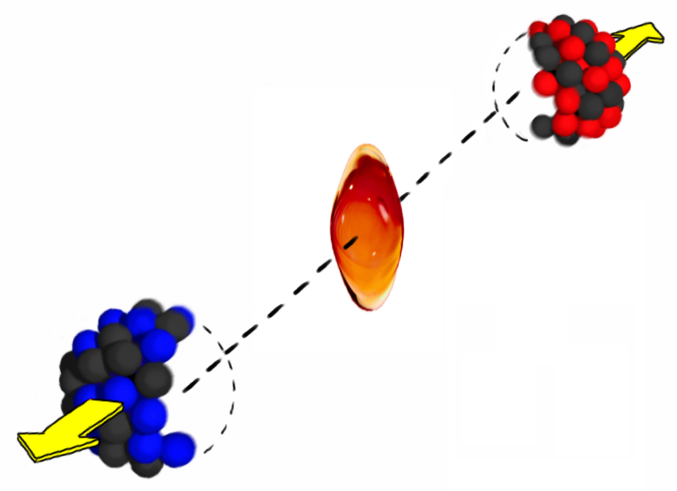
\includegraphics[height=3 cm]{splash.png}

\vspace{-3.7 cm}
\begin{itemize}
\item Heavy ion collisions produce a new kind of fluid \\ called a quark-gluon plasma
\item It survives such a short time that we cannot use \\ traditional methods to study its properties
\item Instead, we look for well-known particle \\ physics processes (``probes'') to see \\ how they are modified by the medium
\item ``Hard'' $\to$ high-energy, perturbative QCD production of dijets, bound states, and electroweak bosons
\end{itemize}

\vspace{-0.5 cm}
\mbox{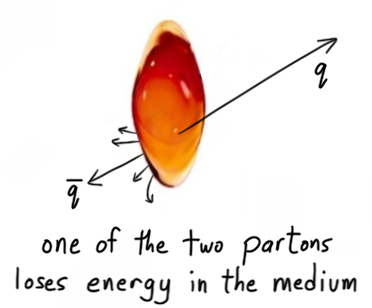
\includegraphics[width=0.33\linewidth]{droplets1.png} 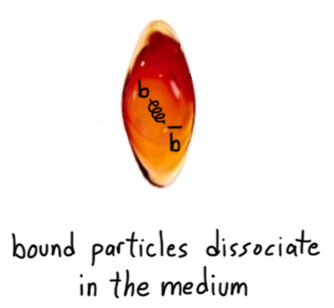
\includegraphics[width=0.33\linewidth]{droplets2.png} 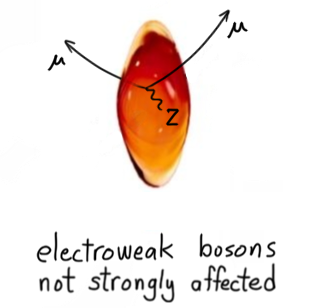
\includegraphics[width=0.33\linewidth]{droplets3.png}}
\end{frame}

\begin{frame}
\frametitle{The CMS detector}

\vspace{0.3 cm}
\begin{columns}
\column{0.68\linewidth}
\centering Minimum Bias and Jet triggers

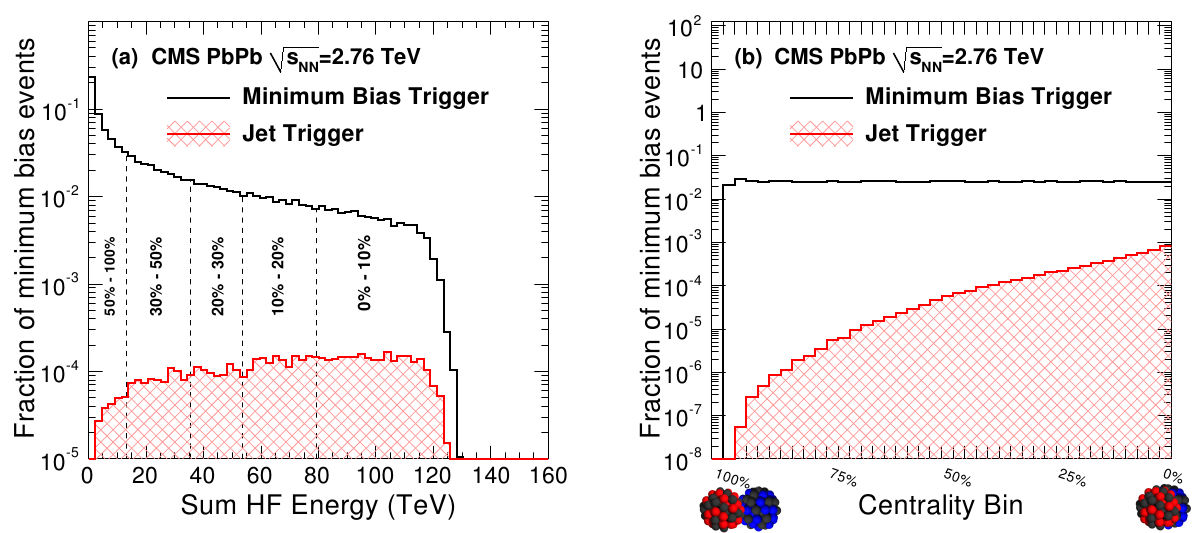
\includegraphics[width=\linewidth]{dijets/trigger_centrality.png}

\column{0.32\linewidth}
\centering Muon efficiency

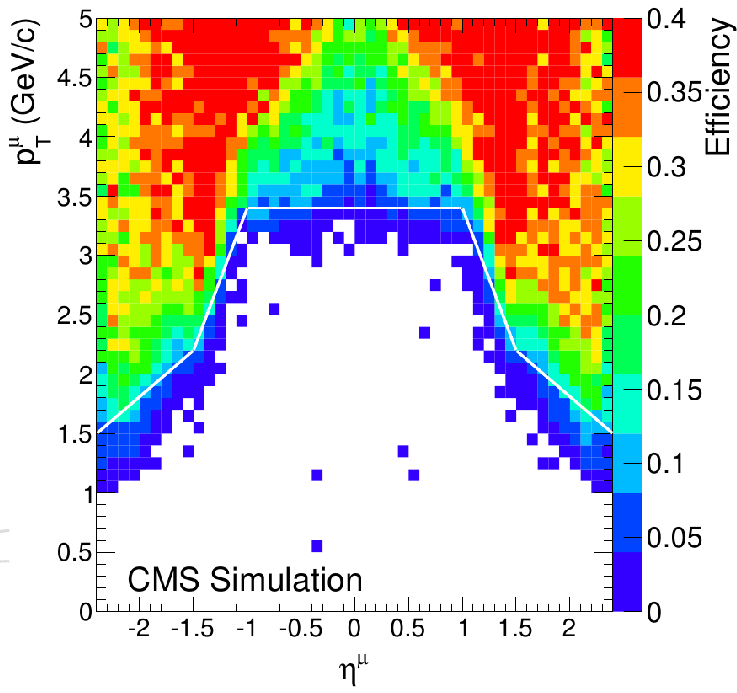
\includegraphics[width=\linewidth]{dimuons/efficiency_pt_eta.png}
\end{columns}

\hfill 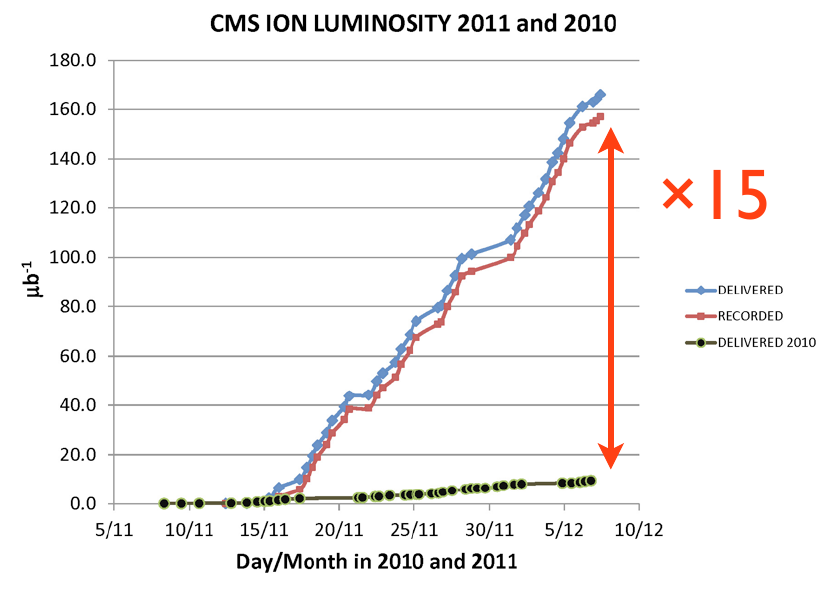
\includegraphics[height=3.5 cm]{intro/luminosity_oldnew.png}

\vspace{-3.5 cm}
\begin{itemize}
\item $\eta$ coverage: $\pm$5.2 for jets, \\ $\pm$2.4 for muons
\item High-resolution tracking up to \\ 100's of GeV
\item Particle flow jets (get charged \\ particle momenta from tracks)
\item 150~$\mu$b$^{-1}$ Pb-Pb {\scriptsize (Nov 2011)} and 231 nb$^{-1}$ of \mbox{2.76~TeV pp {\scriptsize (Mar 2012)}\hspace{-2 cm}}
\end{itemize}
\end{frame}

\begin{frame}
\frametitle{Jet quenching}

\vspace{-0.95 cm}
\hspace{2.3 cm} 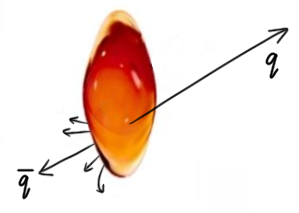
\includegraphics[height=1.5 cm]{droplets1_small.png}

\vspace{-0.55 cm}
\begin{columns}
\column{0.3\linewidth}
\begin{minipage}{2.2\linewidth}
\begin{itemize}
\item Hard process produces two partons, one loses energy in the medium (``quenched'')

\item Dramatic enough at the LHC to see it in event displays

\item Quantify with
\end{itemize}
\end{minipage}

\vspace{-0.3 cm}
\begin{center}
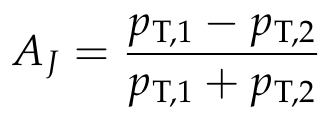
\includegraphics[height=0.7 cm]{dijets/aj_definition.png}

and

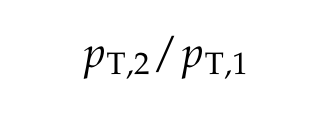
\includegraphics[height=0.7 cm]{dijets/ptratio.png}

\vspace{-0.3 cm}
\end{center}

\vspace{-0.5 cm}
\begin{itemize}
\item Calorimeter-only and particle-flow jet algorithms yield similar results
\end{itemize}

\column{0.7\linewidth}
\vspace{0.5 cm}

\hfill 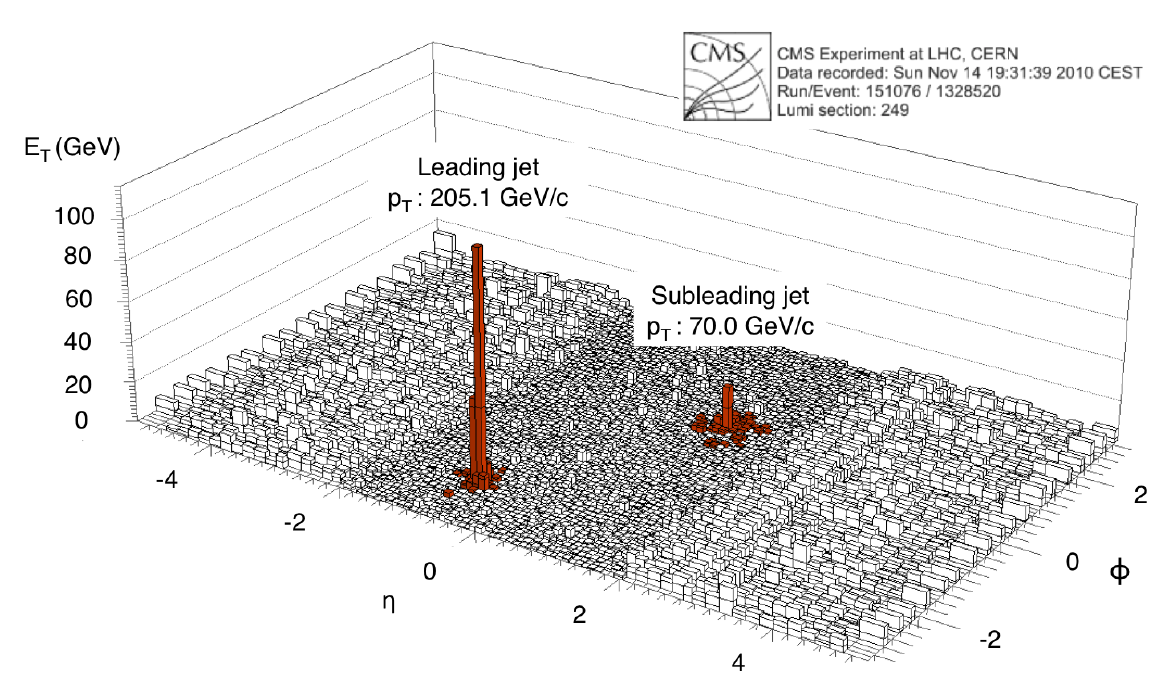
\includegraphics[width=0.5\linewidth]{dijets/eventdisplay.png}

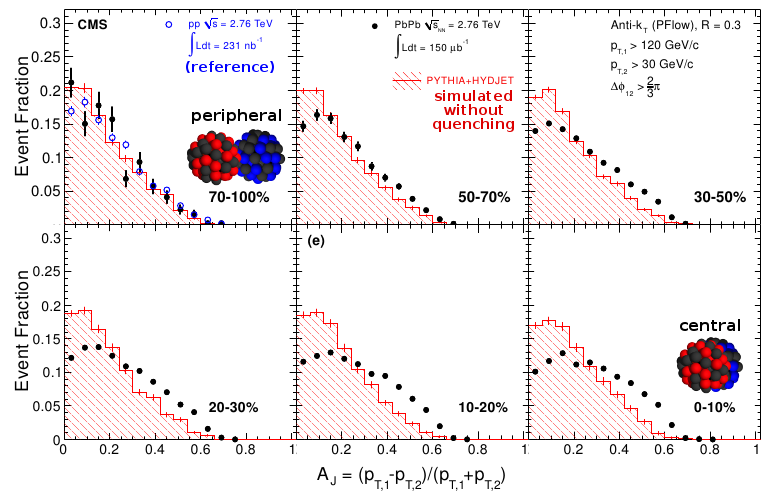
\includegraphics[width=\linewidth]{dijets/asymmetry_ratio.png}
\end{columns}

\vspace{0.2 cm}
\hfill \textcolor{darkblue}{\scriptsize PRC 84 (2011) 024906 \textcolor{black}{and} PLB 712 (2012) 176}

\vspace{-0.2 cm}
\end{frame}

\setbeamertemplate{headline}{\mbox{ } \hfill
\begin{minipage}{5.5 cm}
\vspace{-0.75 cm} \small
\end{minipage} \hfill
\begin{minipage}{4.5 cm}
\vspace{-0.75 cm} \small
\begin{flushright}
\ifthenelse{\equal{\insertpagenumber}{1}}{}{\hspace{0.2 cm} 5\isnote/\pageref{numpages}}
\end{flushright}
\end{minipage}\mbox{\hspace{0.2 cm}}\includegraphics[height=1 cm]{../cmslogo} \hspace{0.01 cm} \vspace{-1.05 cm}}

\begin{frame}
\frametitle{Missing $p_T$ went into \only<-6>{low-$p_T$}\only<7->{large-angle} particles}

\vspace{0.1 cm}
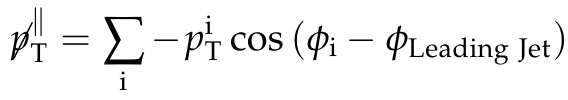
\includegraphics[height=0.7 cm]{dijets/ptmiss_parallel.png}\hspace{0.3 cm}$\begin{array}{c}\mbox{versus} \\ \mbox{ }\end{array}$\hspace{0.3 cm}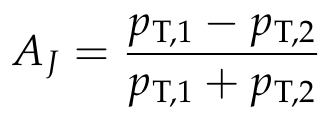
\includegraphics[height=0.7 cm]{dijets/aj_definition.png}

\vspace{-0.6 cm}
\begin{center}
\only<1>{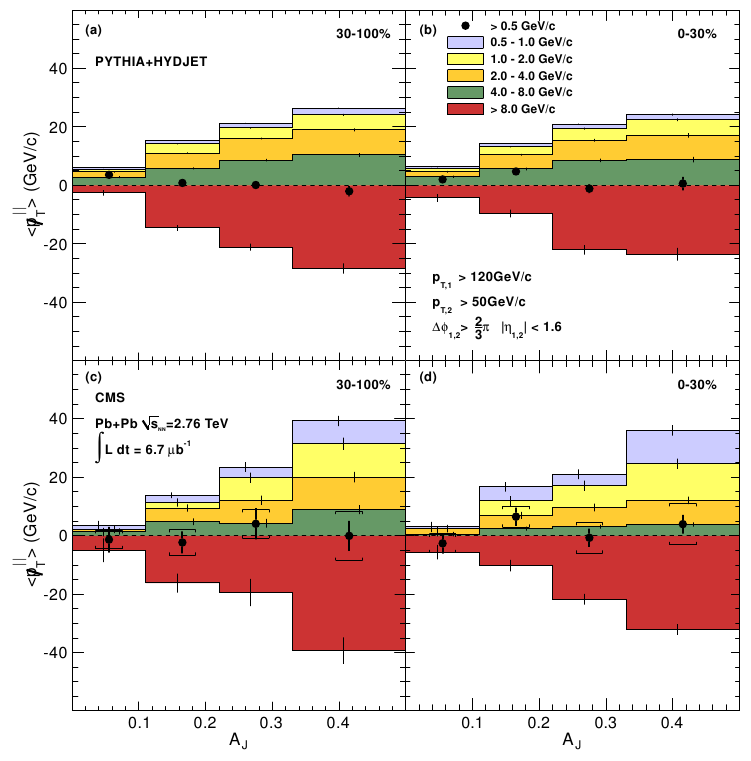
\includegraphics[width=0.7\linewidth]{dijets/restored_balance1.png}}
\only<2>{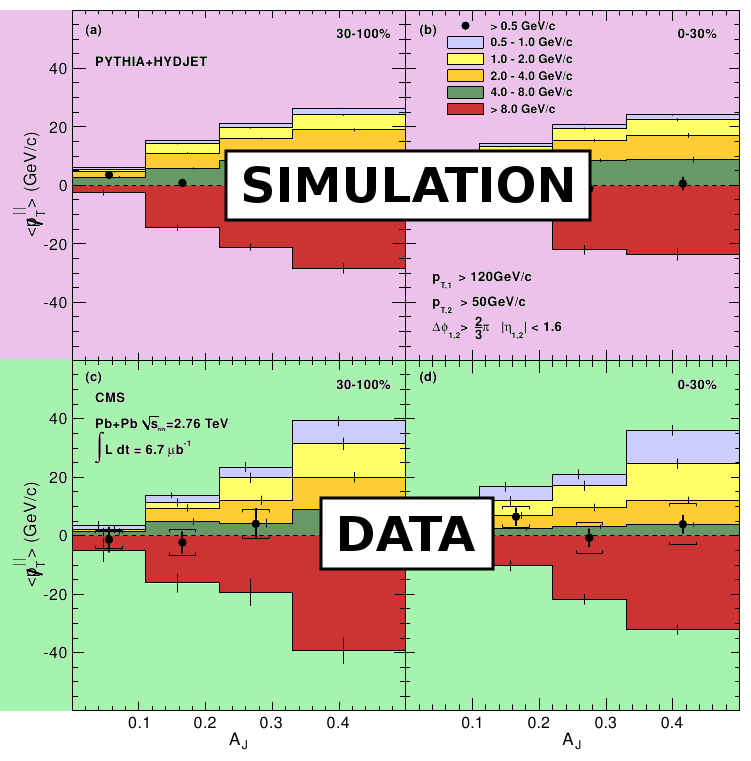
\includegraphics[width=0.7\linewidth]{dijets/restored_balance1_explain1.png}}
\only<3>{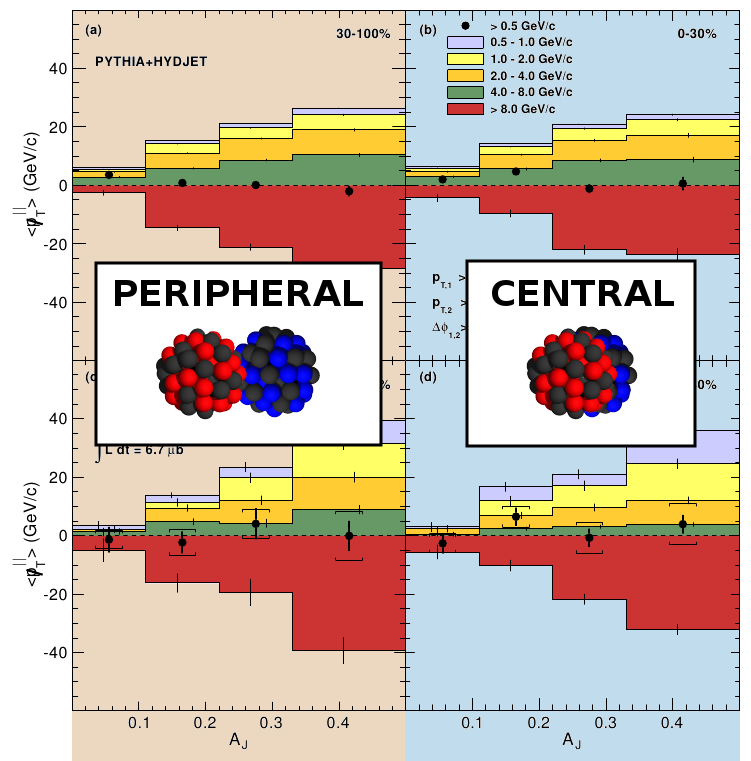
\includegraphics[width=0.7\linewidth]{dijets/restored_balance1_explain2.png}}
\only<4>{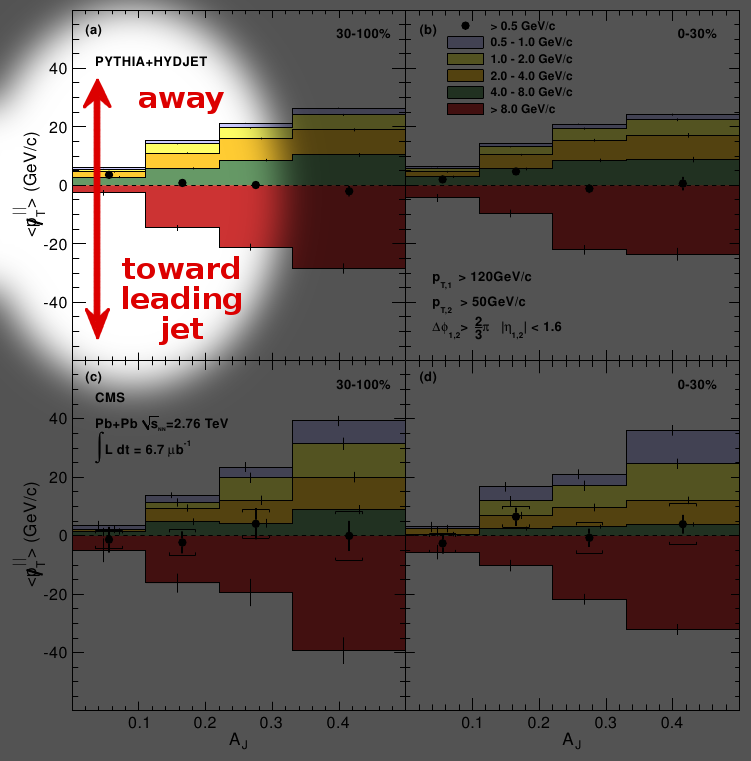
\includegraphics[width=0.7\linewidth]{dijets/restored_balance1_explain3.png}}
\only<5>{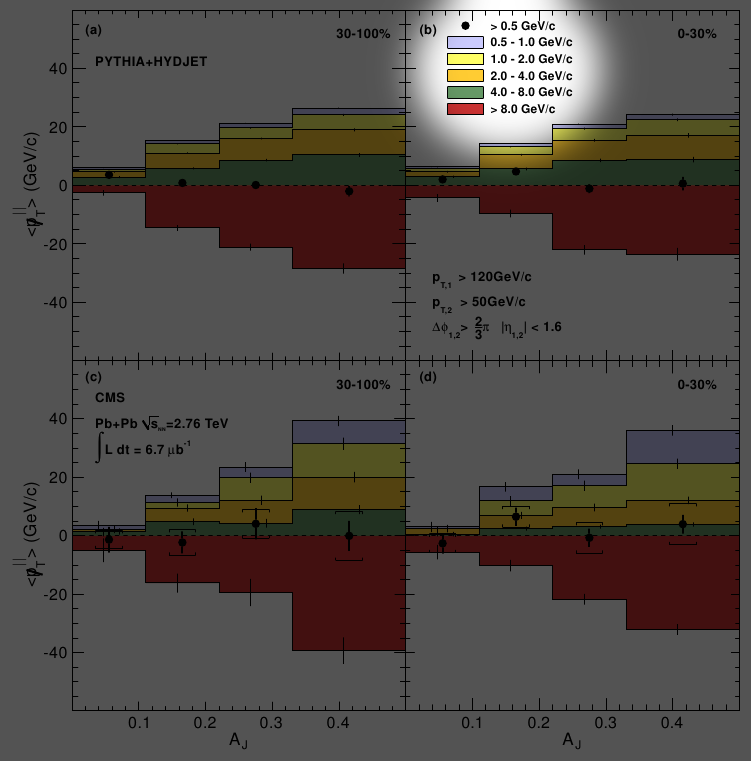
\includegraphics[width=0.7\linewidth]{dijets/restored_balance1_explain4.png}}
\only<6>{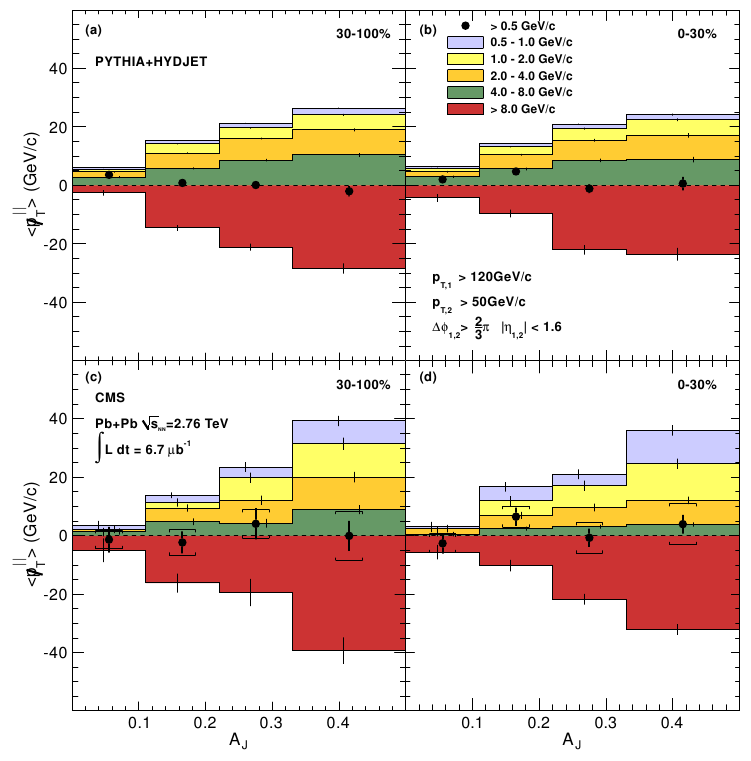
\includegraphics[width=0.7\linewidth]{dijets/restored_balance1.png}}
\only<7>{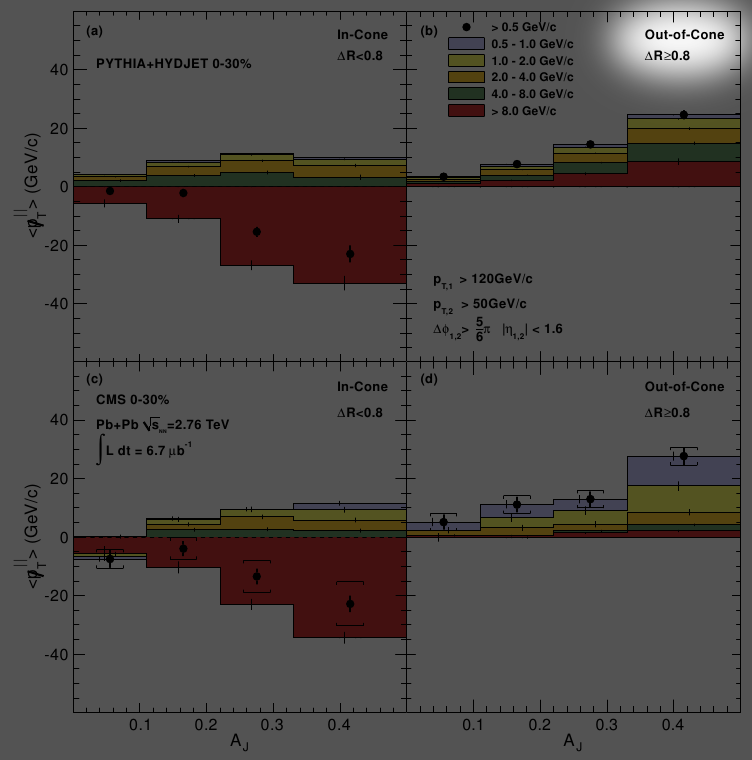
\includegraphics[width=0.7\linewidth]{dijets/restored_balance2_explain1.png}}
\only<8>{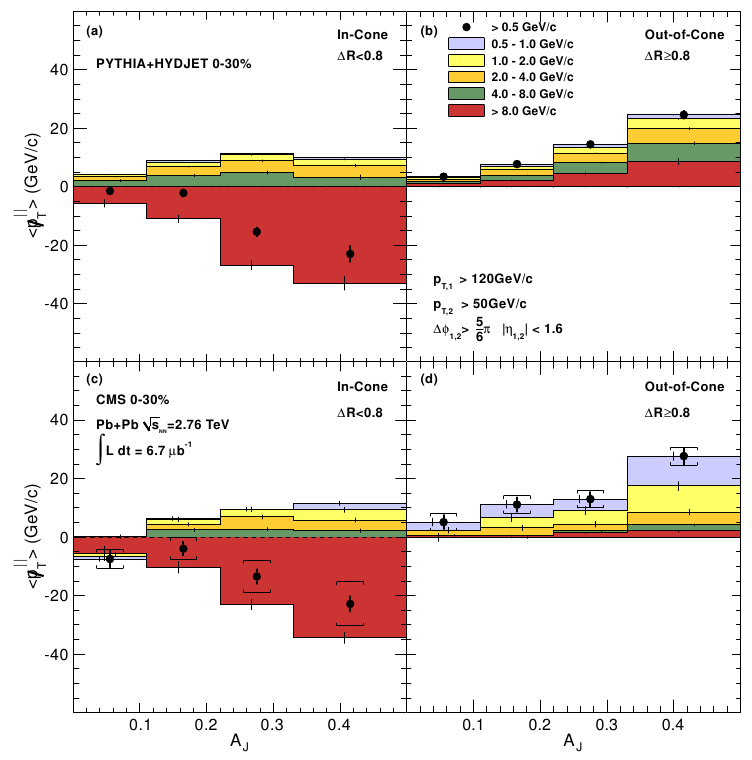
\includegraphics[width=0.7\linewidth]{dijets/restored_balance2.png}}
\end{center}

\vspace{-0.6 cm} \scriptsize
\hfill \textcolor{darkblue}{\mbox{PRC 84 (2011) 024906\hspace{-0.5 cm}}}
\end{frame}

\setbeamertemplate{headline}{\mbox{ } \hfill
\begin{minipage}{5.5 cm}
\vspace{-0.75 cm} \small
\end{minipage} \hfill
\begin{minipage}{4.5 cm}
\vspace{-0.75 cm} \small
\begin{flushright}
\ifthenelse{\equal{\insertpagenumber}{1}}{}{Jim Pivarski \hspace{0.2 cm} \insertpagenumber\isnote/\pageref{numpages}}
\end{flushright}
\end{minipage}\mbox{\hspace{0.2 cm}}\includegraphics[height=1 cm]{../cmslogo} \hspace{0.01 cm} \vspace{-1.05 cm}}

\setcounter{page}{6}

\begin{frame}
\frametitle{Negligible dependence on leading $p_T$}

\begin{itemize}
\item vertical axis: $\displaystyle \frac{\mbox{subleading } p_T}{\mbox{leading } p_T}$ fraction, horizontal axis: leading $p_T$
\end{itemize}

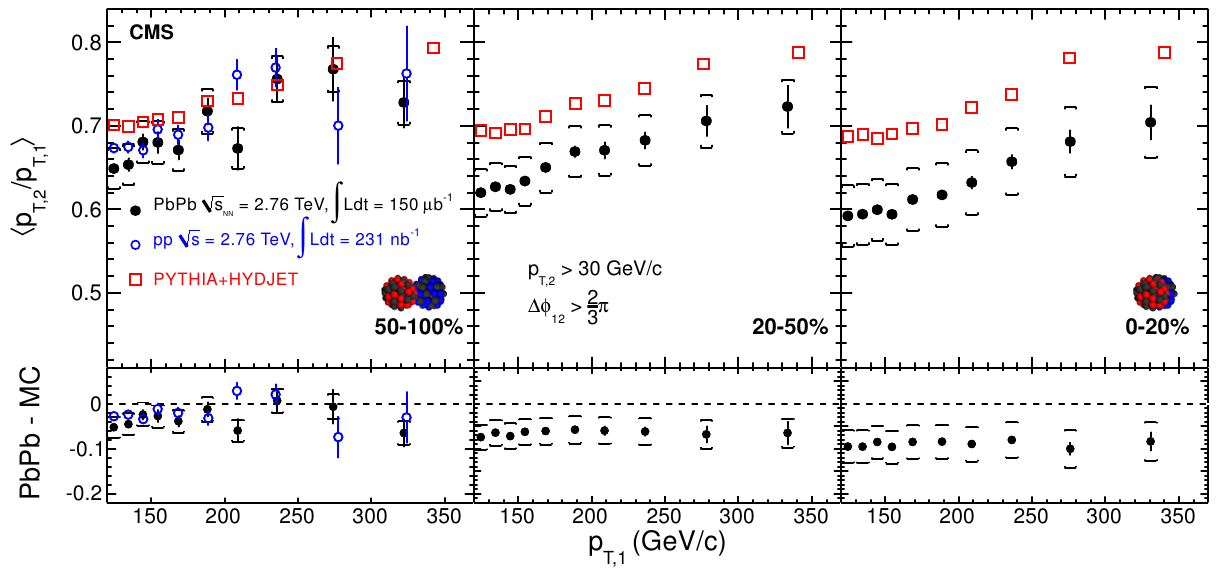
\includegraphics[width=\linewidth]{dijets/quench_vs_pt.png}

\hfill \textcolor{darkblue}{\scriptsize PLB 712 (2012) 176}
\end{frame}

\begin{frame}
\frametitle{Negligible angle decorrelation}

\begin{columns}
\column{0.35\linewidth}

\begin{itemize}
\item Photon-jet pairs produced in $qg \to \gamma q$ and $q\bar{q} \to
  \gamma g$
\item The photon does not interact with the medium, making it a good
  probe of the initial state of the parton that produced the jet
\item Dijets and photon-jet correlations both show large energy
  loss, rather than angle decorrelation
\end{itemize}

\column{0.65\linewidth}

\centering dijet angular distributions

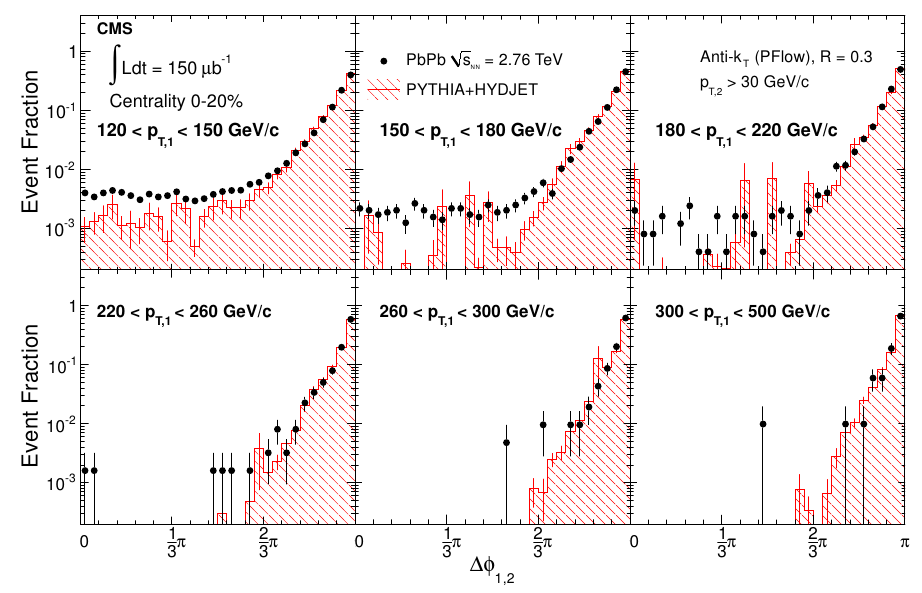
\includegraphics[width=\linewidth]{dijets/angles_dijets.png}

\vspace{-0.2 cm}
\centering \textcolor{darkblue}{\scriptsize PLB 712 (2012) 176}

\vspace{0.2 cm}
\centering $\gamma$-jet angular distributions

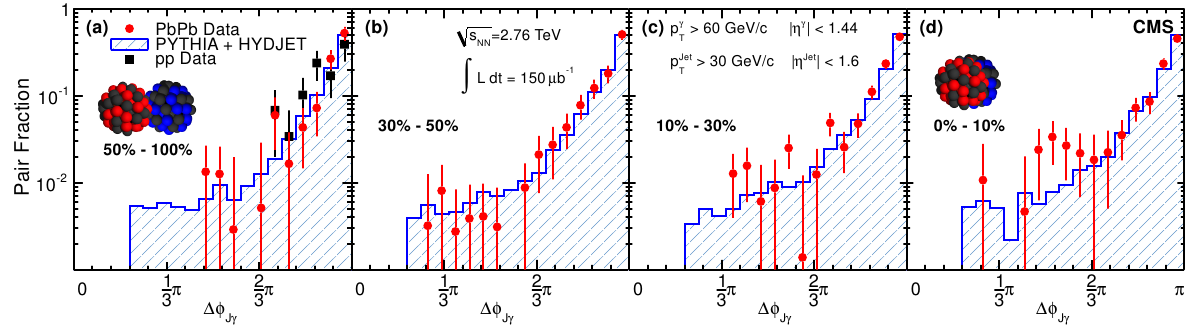
\includegraphics[width=\linewidth]{dijets/angles_gammajets.png}

% 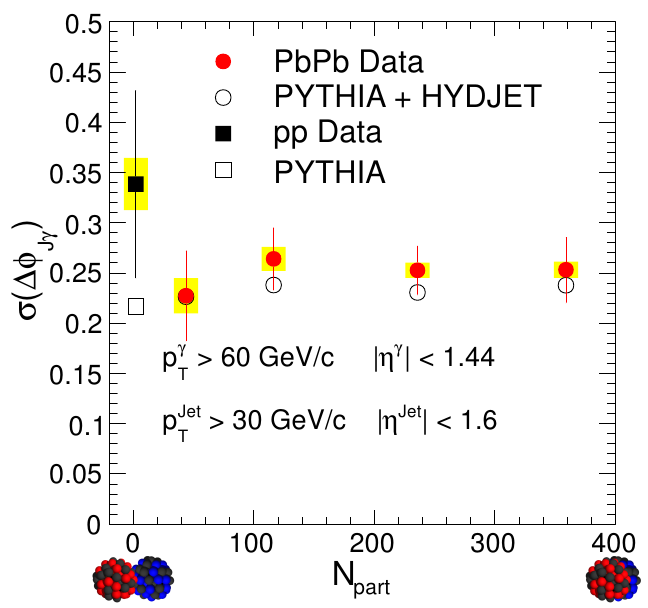
\includegraphics[width=0.5\linewidth]{dijets/angles_gammajets2.png}

\vspace{-0.2 cm}
\centering \textcolor{darkblue}{\scriptsize arXiv:1205.0206, submitted to PLB}
\end{columns}

\end{frame}

\begin{frame}
\frametitle{Quarkonia $\to \mu\mu$}

\vspace{-1.5 cm}
\hspace{3 cm} 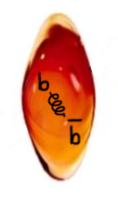
\includegraphics[height=1.5 cm]{droplets2_small.png}

\vspace{0.5 cm}

\begin{columns}
\column{0.6\linewidth}
Dimuon spectrum in 2011 heavy ions

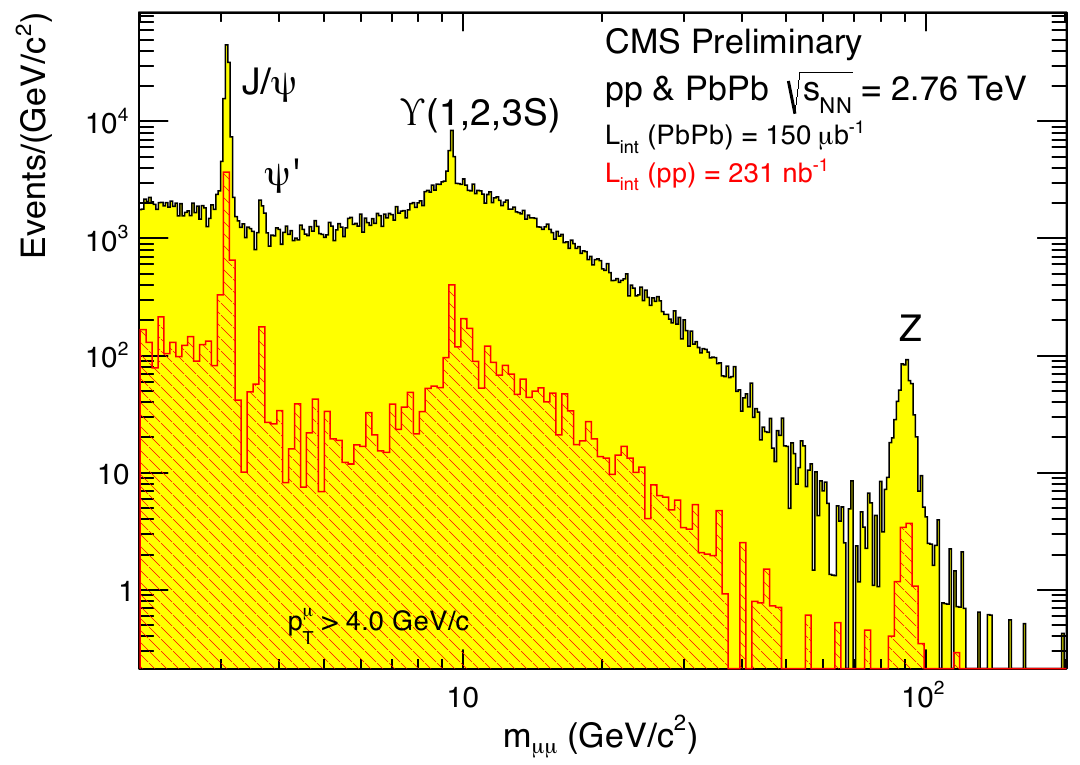
\includegraphics[width=\linewidth]{dimuons/dimuons_2011.png}

\column{0.4\linewidth}
Upsilon candidate

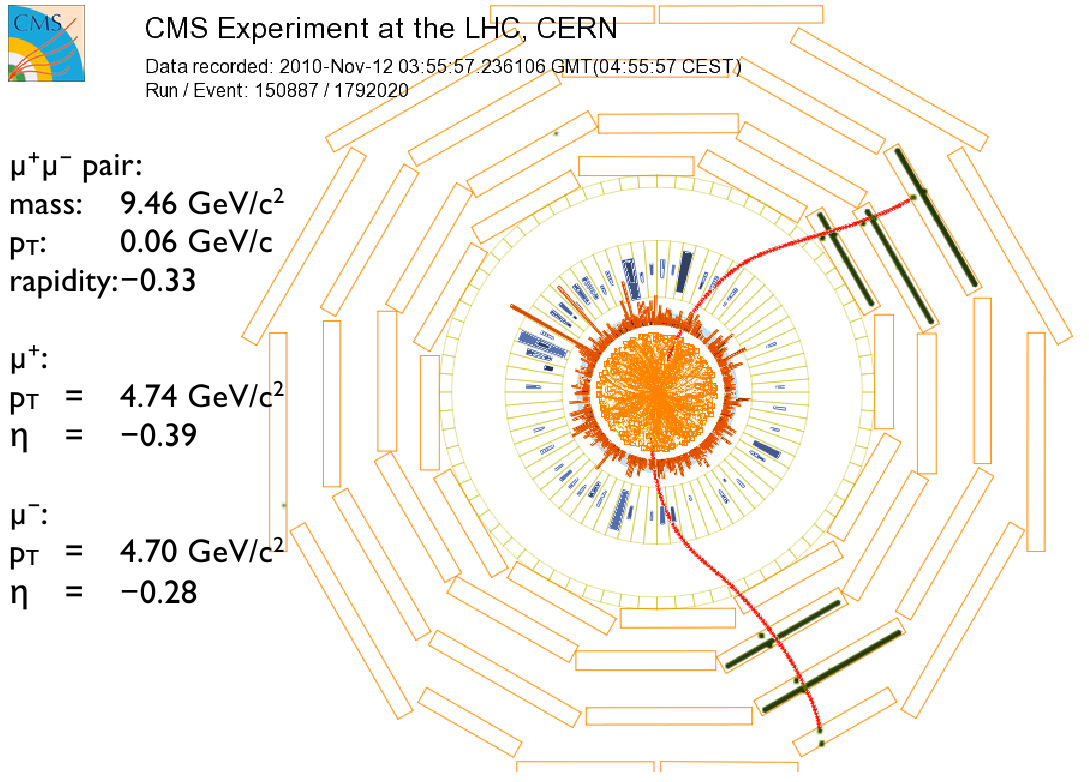
\includegraphics[width=\linewidth]{dimuons/upsilon_eventdisplay.png}

\vspace{0.5 cm}
Tag-and-probe example plot

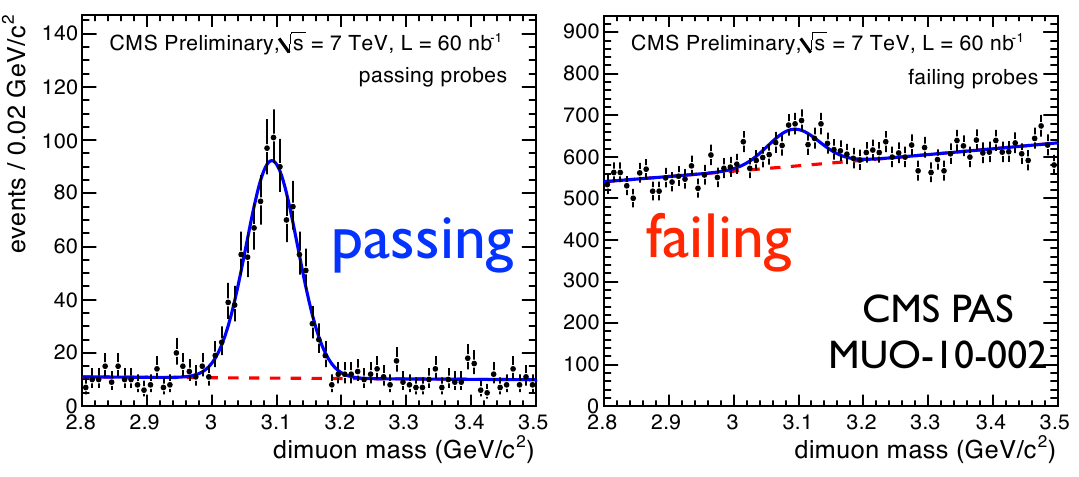
\includegraphics[width=\linewidth]{dimuons/muon_tag_and_probe.png}
%% 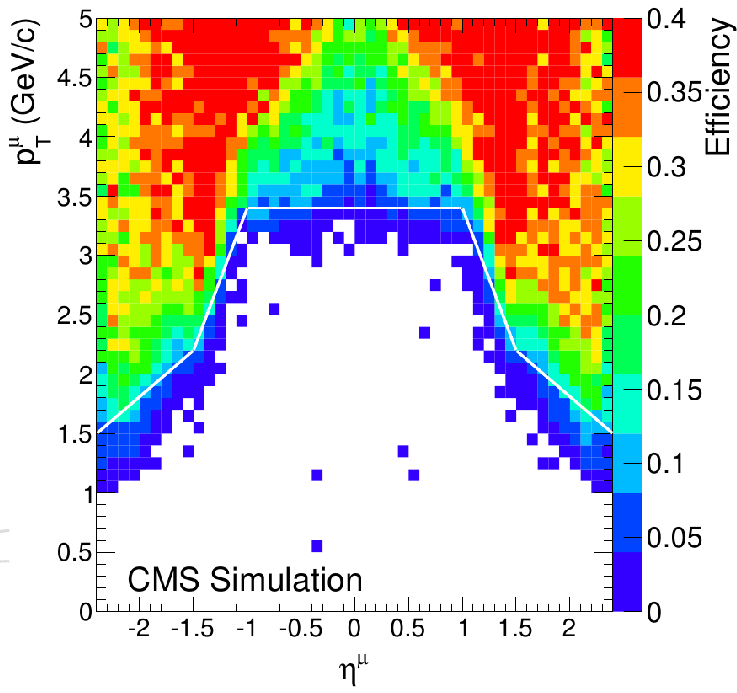
\includegraphics[width=0.2\linewidth]{dimuons/efficiency_pt_eta.png}
\end{columns}
\end{frame}

\begin{frame}
\frametitle{Upsilon suppression, state by state}

\begin{columns}
\column{0.6\linewidth}
\vspace{0.5 cm}
\only<1>{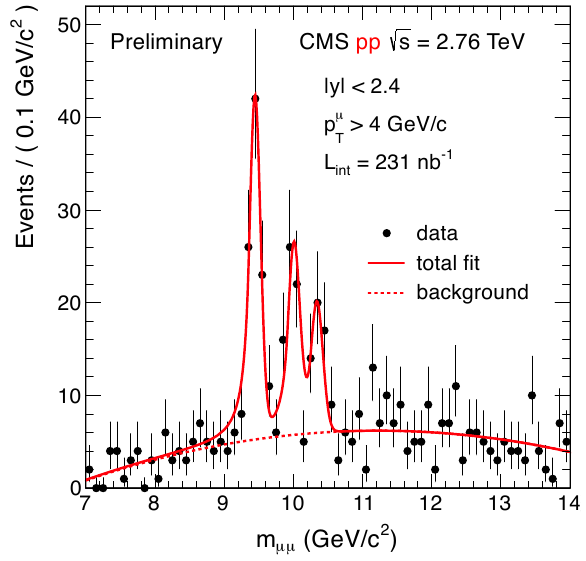
\includegraphics[width=\linewidth]{dimuons/upsilons_pp.png}}
\only<2>{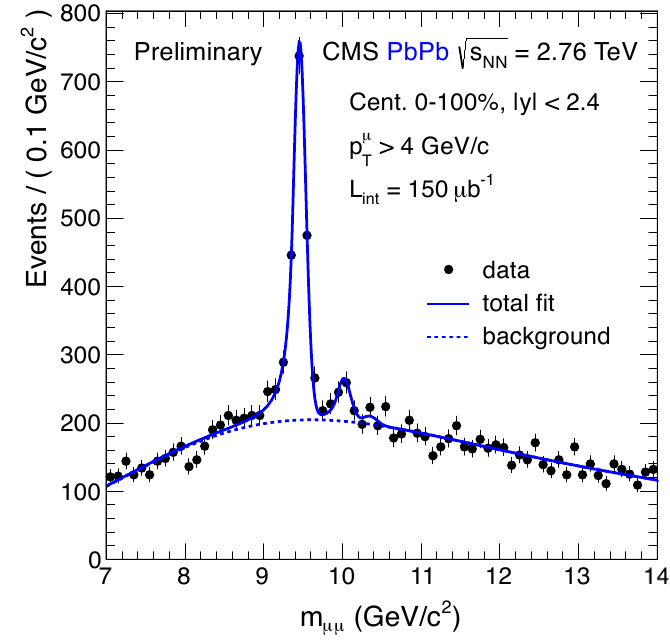
\includegraphics[width=\linewidth]{dimuons/upsilons_pb_pb.png}}
\only<3>{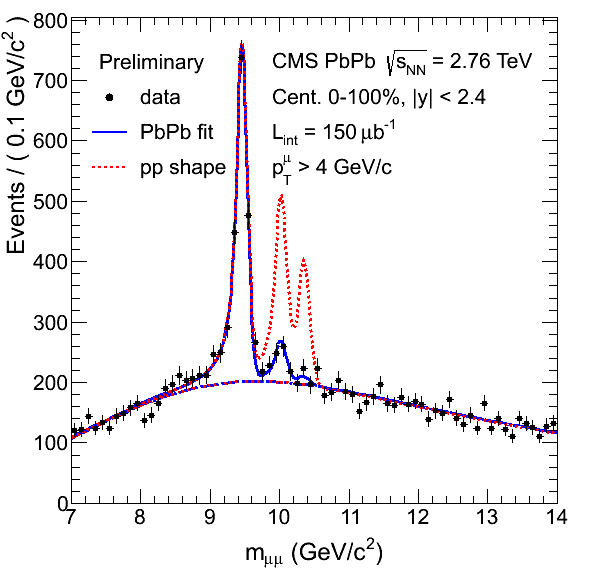
\includegraphics[width=\linewidth]{dimuons/upsilons_overlay.png}}

\column{0.4\linewidth}
\vspace{-0.5 cm}
\begin{itemize}
\item CMS can resolve the three $\Upsilon$ states
\item<2-> In heavy ion collisions, all are suppressed, but $\Upsilon(2S)$ and $\Upsilon(3S)$ more than $\Upsilon(1S)$
\item<3-> Significance of suppression: 5.4$\sigma$
\item<3-> Double ratio \scriptsize \mbox{$\displaystyle \frac{\left.nS/1S\right|_{\mbox{\tiny Pb$\,$Pb}}}{\left.nS/1S\right|_{\mbox{\tiny pp}}}$\hspace{-0.5 cm}} \\

2S/1S = $0.21 \pm 0.07 \pm 0.02$ \\
3S/1S $<$ 0.1 (95\% C.L.)
\end{itemize}
\end{columns}

\scriptsize
\hfill \textcolor{darkblue}{PRL 107 (2011) 052302}

\hfill \textcolor{darkblue}{https://twiki.cern.ch/twiki/bin/view/CMSPublic/PhysicsResultsHIN11011}
\end{frame}

\begin{frame}
\frametitle{No clear dependence on centrality}
\begin{center}
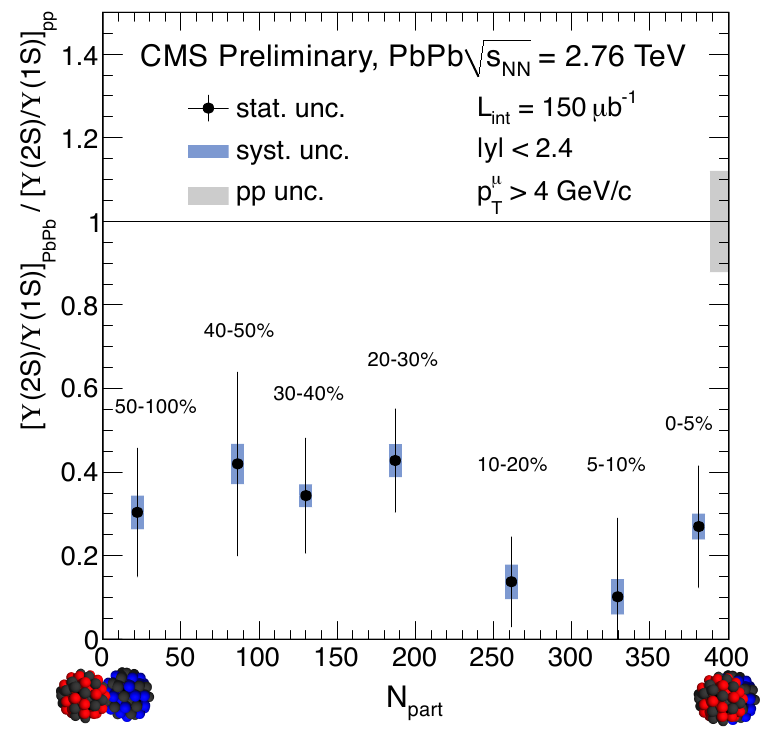
\includegraphics[width=0.75\linewidth]{dimuons/upsilon_doubleratio_centrality.png}
\end{center}
\end{frame}

\begin{frame}
\frametitle{J/$\psi$ suppression measured for prompt \\ and non-prompt samples}

\begin{columns}
\column{0.7\linewidth}
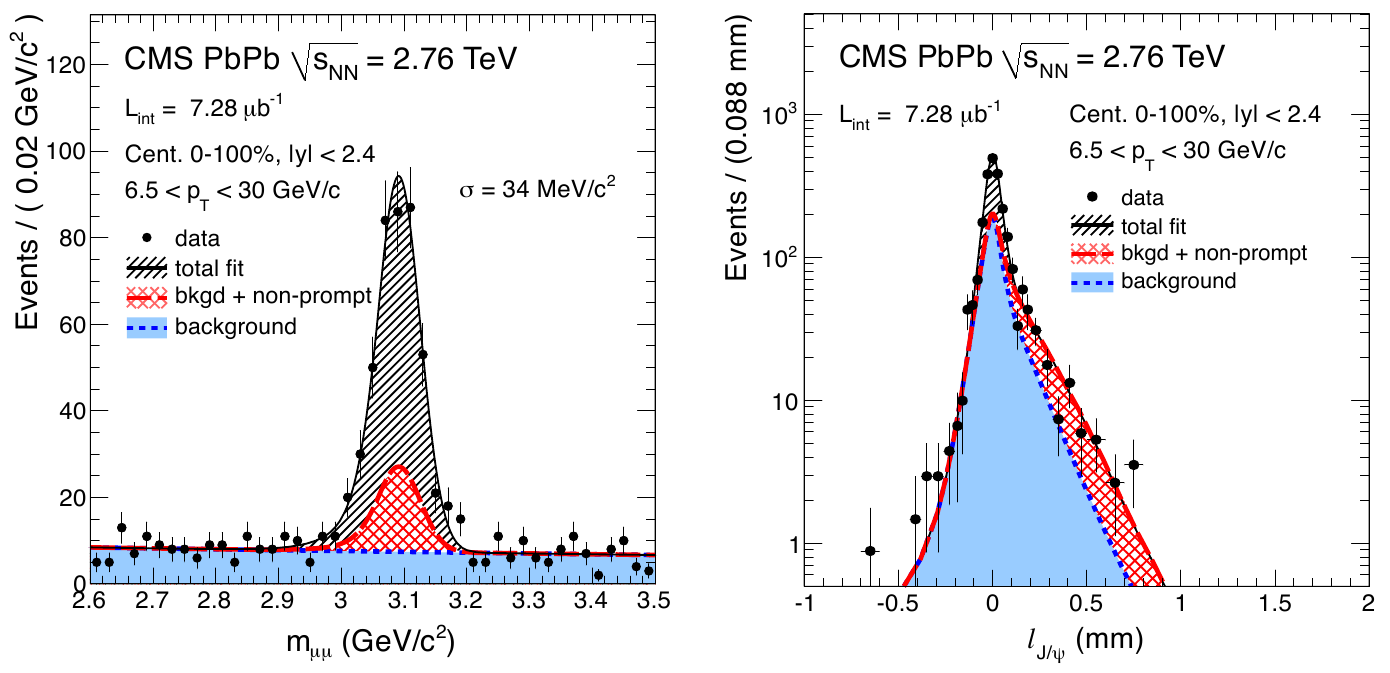
\includegraphics[width=\linewidth]{dimuons/jpsi_prompt_nonprompt.png}

\column{0.35\linewidth}
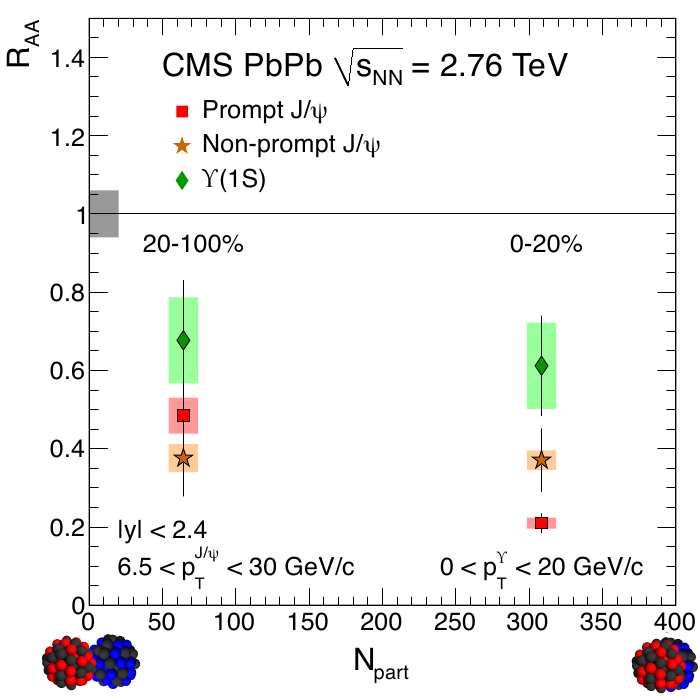
\includegraphics[width=\linewidth]{dimuons/jpsi_prompt_nonprompt_centrality.png}
\end{columns}

\begin{itemize}
\item In $B \to J/\psi \, X$, the secondary vertex from the long-lived $B$, far from the quark-gluon plasma, can be distinguished from prompt $J/\psi$ production
\item $l_{\mbox{\scriptsize J/$\psi$}}$ is the proper flight distance along the dimuon momentum axis ($l_{\mbox{\scriptsize J/$\psi$}} < 0$ part of the distribution is purely resolution)
\item $\displaystyle R_{AA} = \frac{\mathcal{L}_{\mbox{\scriptsize pp}}}{T_{AA}N_{\mbox{\scriptsize MB}}} \frac{N_{\mbox{\scriptsize PbPb}}(Q\bar{Q})}{N_{\mbox{\scriptsize pp}}(Q\bar{Q})} \cdot \frac{\varepsilon_{\mbox{\scriptsize pp}}}{\varepsilon_{\mbox{\scriptsize PbPb}}}$, the \mbox{nuclear modification factor\hspace{-1 cm}}
\end{itemize}

\vspace{-0.3 cm}
\hfill \textcolor{darkblue}{\scriptsize JHEP 1205 (2012) 063}
\end{frame}

\begin{frame}
\frametitle{Matsui-Satz screening}

\vspace{-0.2 cm}
\begin{itemize}
\item Suppression of $\Upsilon(1S)$, prompt $J/\psi$, $\Upsilon(2S)$, and $\Upsilon(3S)$ follow the pattern of their binding energies
\item Supports the idea that the medium is screening their potentials
\end{itemize}

\begin{columns}
\column{0.7\linewidth}
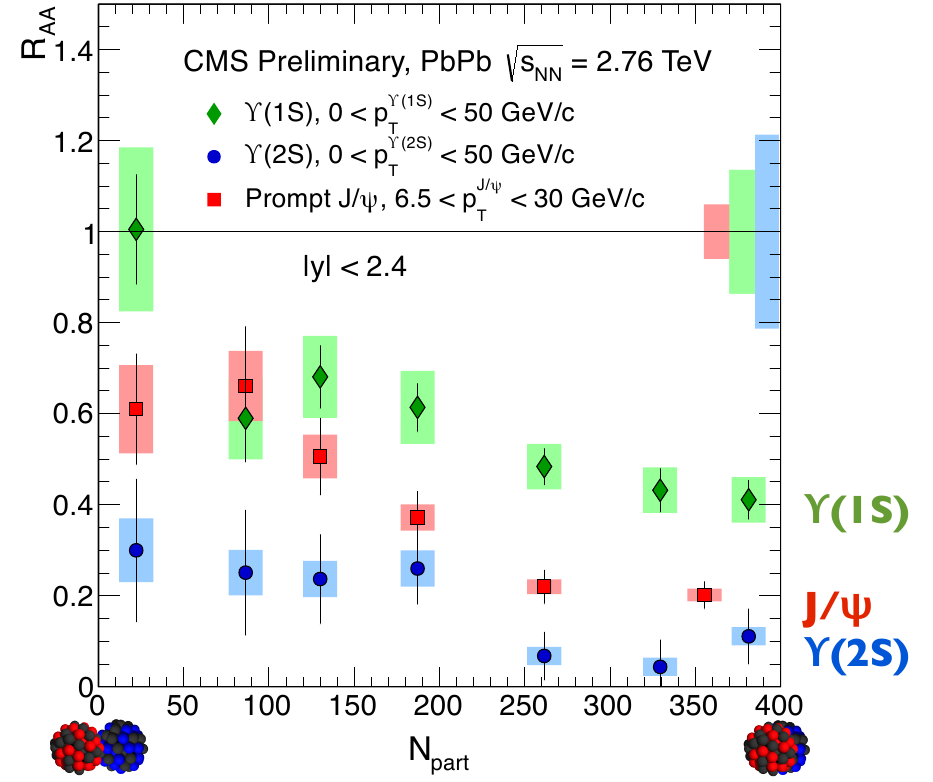
\includegraphics[width=\linewidth]{dimuons/quarkonia_raa_centrality.png}

\column{0.3\linewidth}
%% 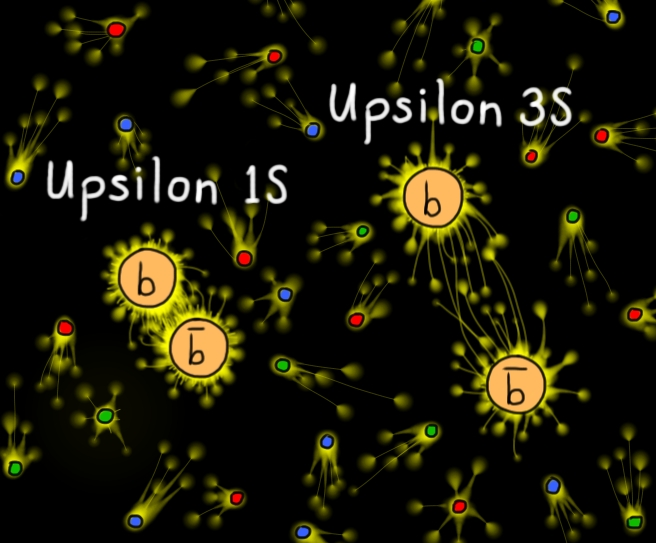
\includegraphics[width=0.2\linewidth]{dimuons/blobs.jpg}
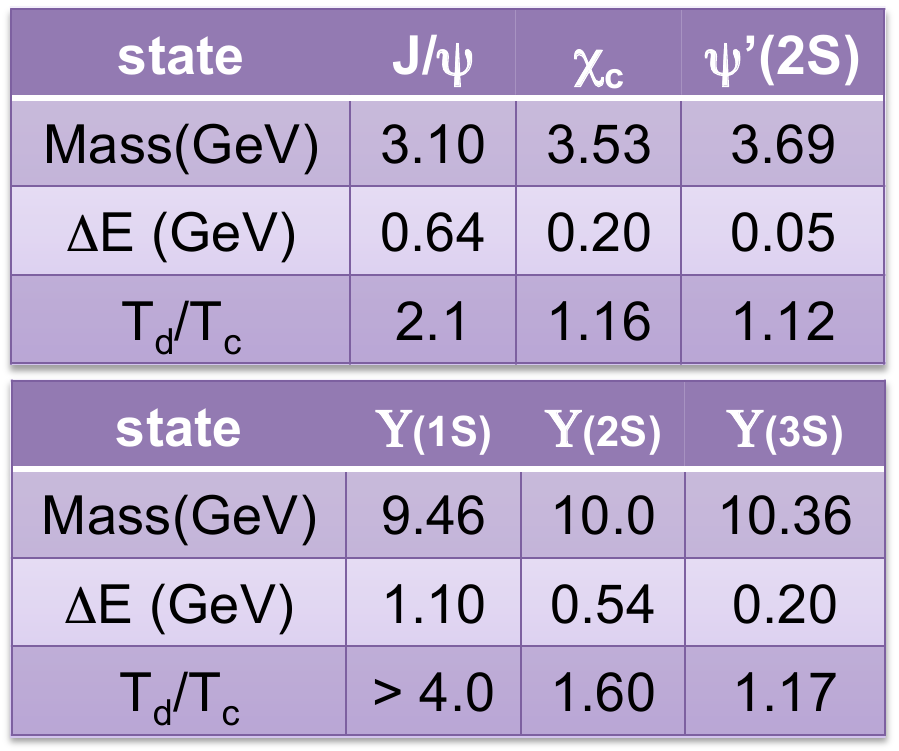
\includegraphics[width=\linewidth]{dimuons/thermometer_table.png}

\vspace{0.2 cm}
\hfill 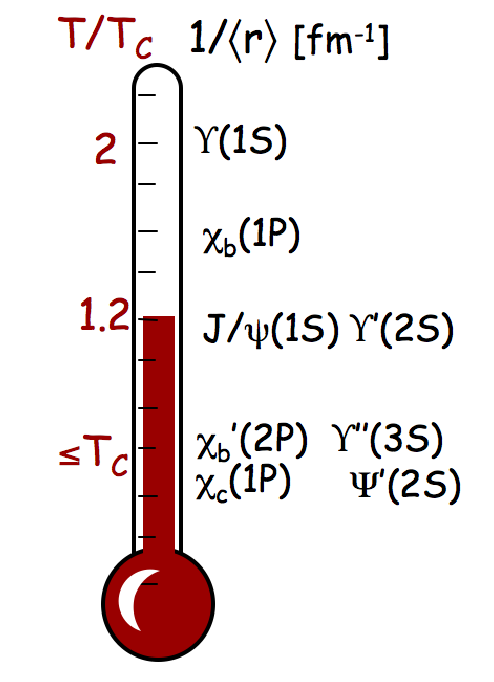
\includegraphics[width=0.75\linewidth]{dimuons/thermometer.png}
\end{columns}

\hfill \textcolor{darkblue}{\scriptsize PLB 178, 416 (1986)}
\end{frame}

\begin{frame}
\frametitle{New: $\psi(2S)$-to-$J/\psi$ double ratio}

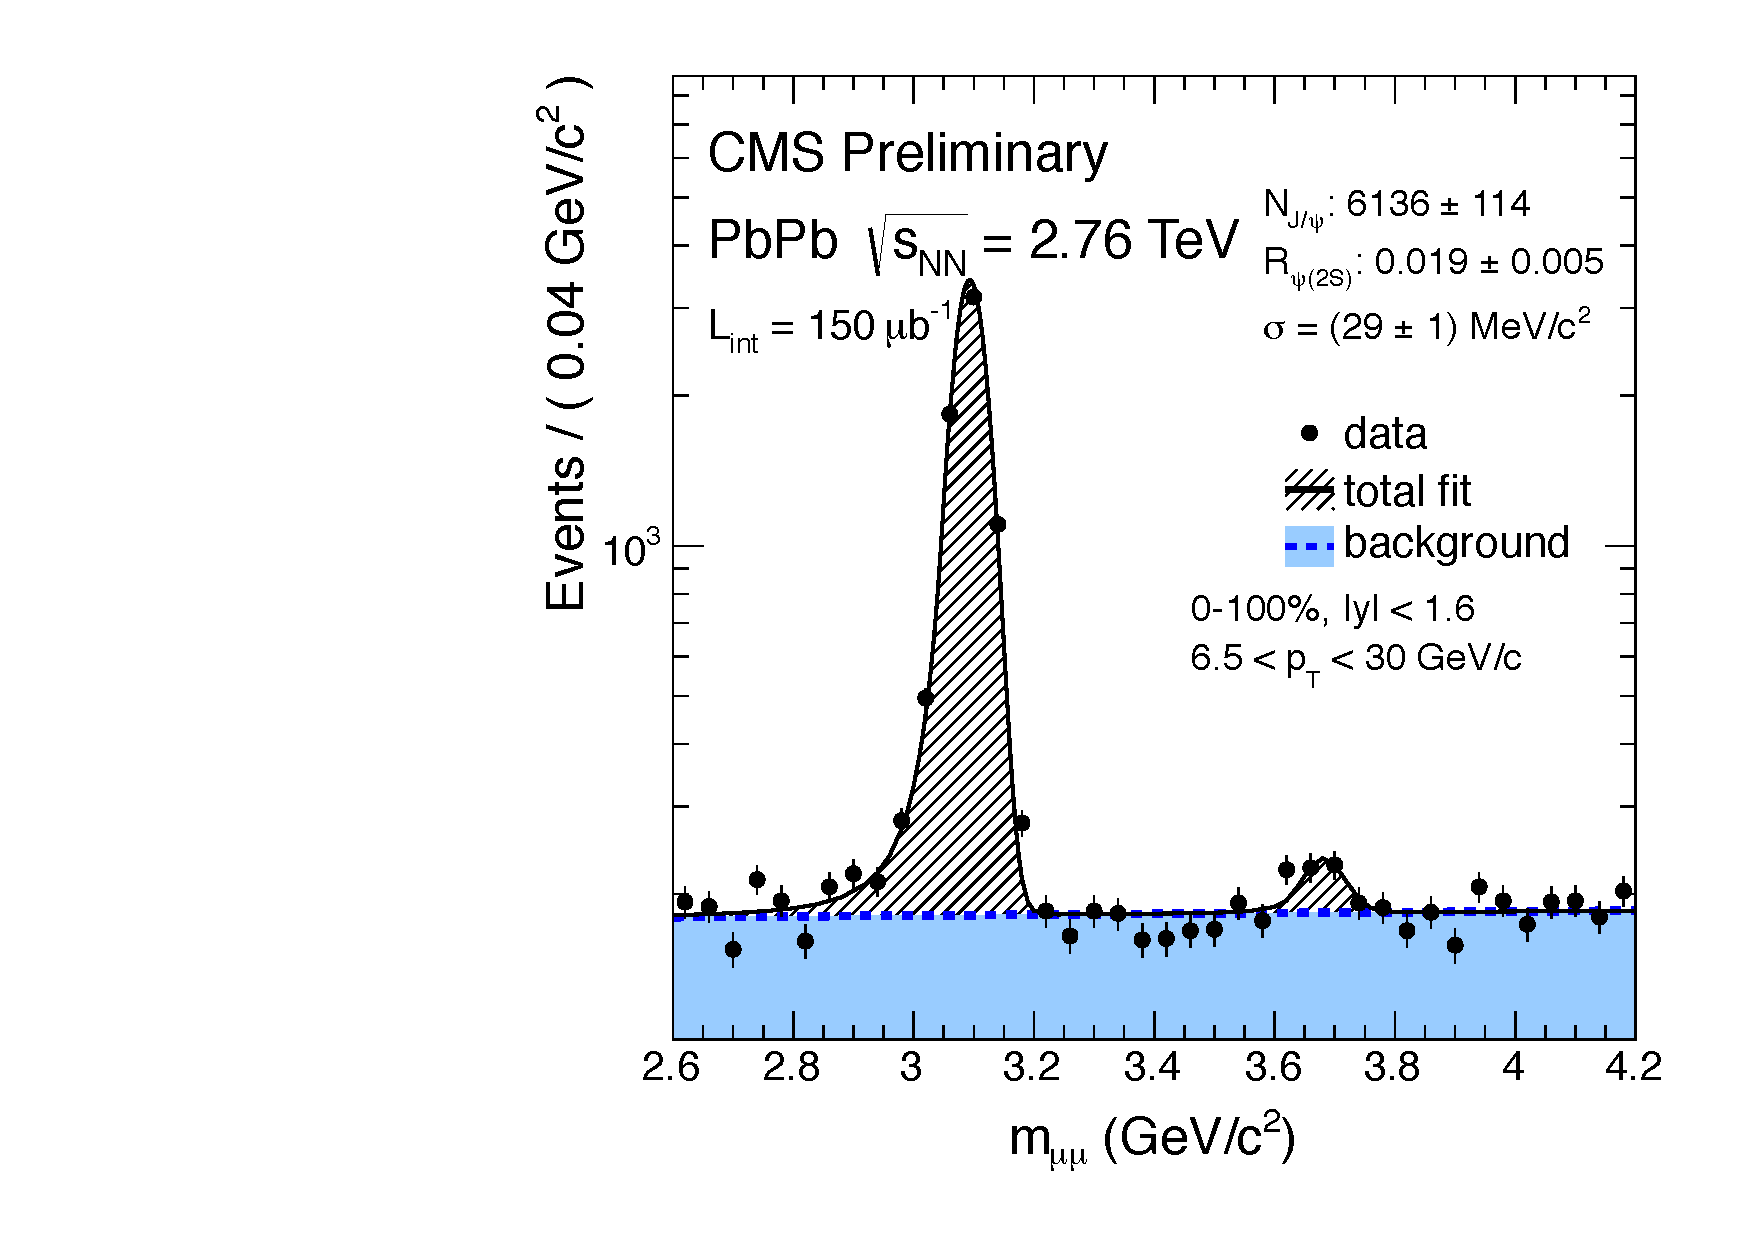
\includegraphics[height=4.2 cm]{dimuons/psi2s.pdf}
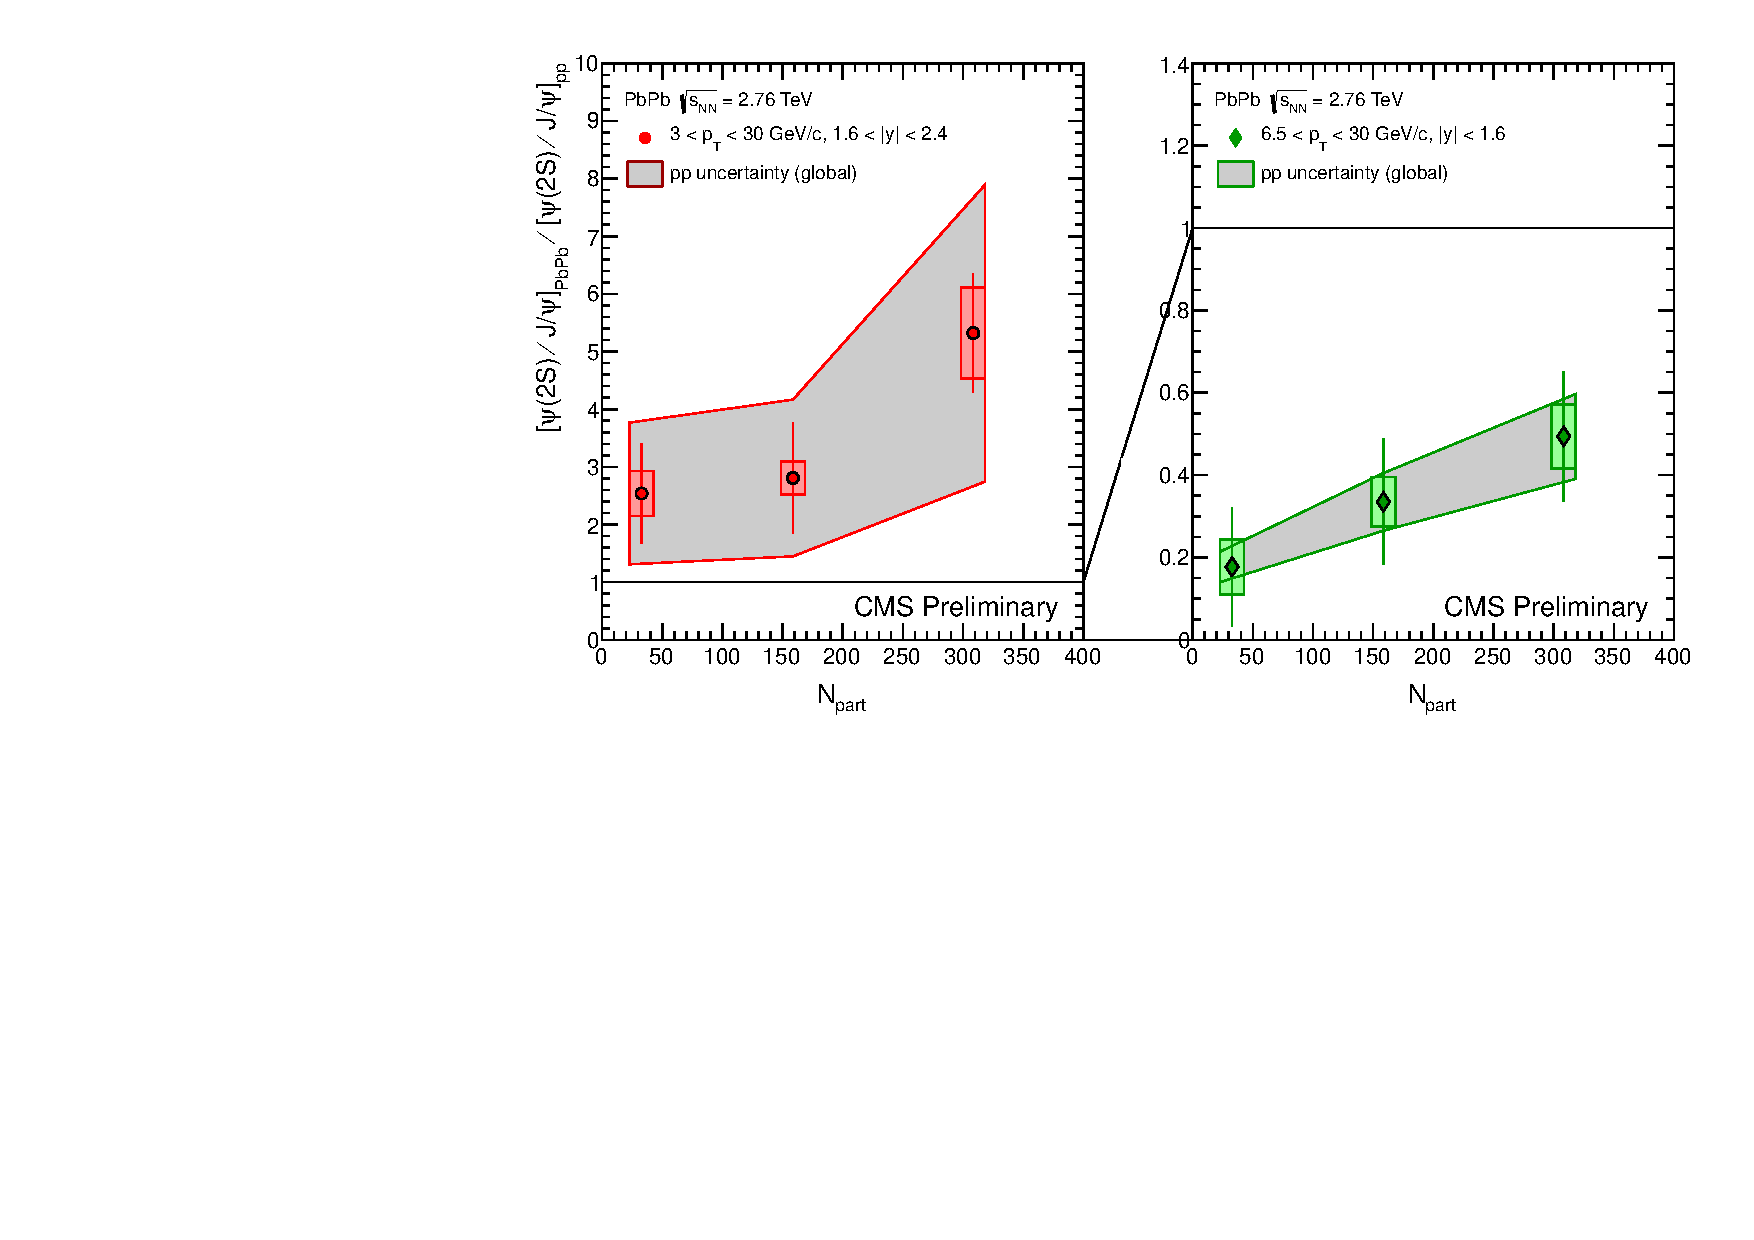
\includegraphics[height=4.2 cm]{dimuons/double_ratio_ppGlobal_midpt_slides.pdf}

\begin{itemize}
\item $J/\psi$ appears more suppressed than $\psi(2S)$ \mbox{in \textcolor{red}{forward, low $p_T$ region}\hspace{-1 cm}}
\item $\psi(2S)$ is more suppressed than $J/\psi$ \mbox{at \textcolor{darkgreen}{midrapidity, higher $p_T$}\hspace{-1 cm}}

\item Note, however, that uncertainties (mostly from pp reference) are large: the highest point is

5.32 $\pm$ 1.03 (stat.) $\pm$ 0.79 (syst.) $\pm$ 2.58 (pp), or 1.5 \mbox{sigma from unity\hspace{-1 cm}}

\end{itemize}

\scriptsize
\hfill \textcolor{darkblue}{https://twiki.cern.ch/twiki/bin/view/CMSPublic/PhysicsResultsHIN12007}
\end{frame}

\begin{frame}
\frametitle{Colorless probes are unaffected}

\vspace{-0.75 cm}
\hspace{5.6 cm} 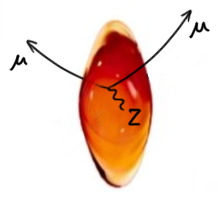
\includegraphics[height=1.5 cm]{droplets3_small.png}

\vspace{-0.5 cm}

\begin{columns}
\column{0.45\linewidth}
\centering isolated photons

\centering 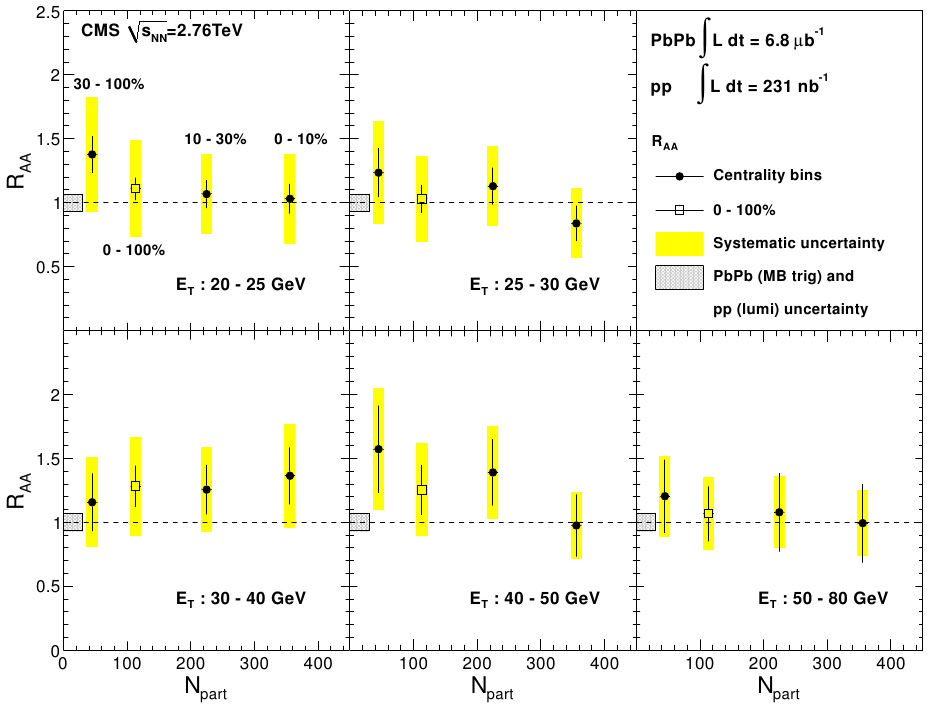
\includegraphics[width=0.93\linewidth]{dijets/photon_raa_centrality.png}

\centering \textcolor{darkblue}{\scriptsize PLB 710 (2012) 256}

\column{0.05\linewidth}

\column{0.42\linewidth}
\centering $Z \to \mu \mu$

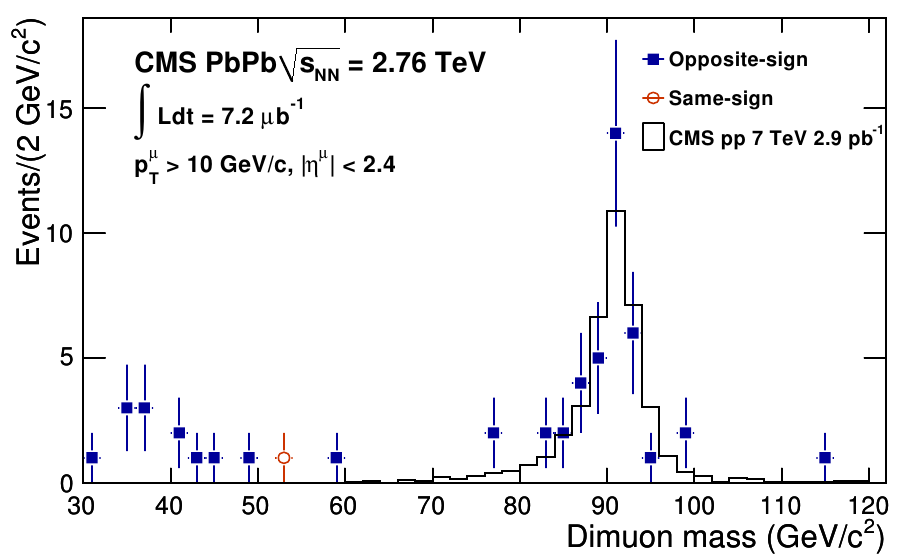
\includegraphics[width=\linewidth]{dimuons/z_mass.png}

\centering \textcolor{darkblue}{\scriptsize PRL 106 (2011) 212301}
\end{columns}

\begin{columns}
\column{0.84\linewidth}
\centering $W \to \mu \nu$

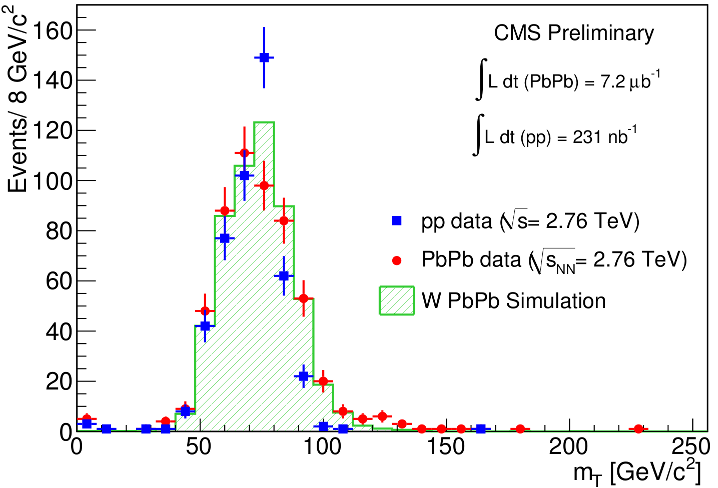
\includegraphics[width=0.5\linewidth]{dimuons/w_mass.png}

\centering \textcolor{darkblue}{\scriptsize arXiv:1205.6334, submitted to PLB}
\end{columns}
\end{frame}

\begin{frame}
\frametitle{Colorless probes are unaffected}
\begin{center}
\includegraphics[width=0.8\linewidth]{dimuons/RAAs-Boson-8.png}
\end{center}
\end{frame}

%% \section*{First section}
%% \begin{frame}
%% \begin{center}
%% \Huge \textcolor{blue}{First section}
%% \end{center}
%% \end{frame}

\begin{frame}
\frametitle{Conclusions}

\begin{itemize}
\item Jet quenching:
\begin{itemize}
\item Asymmetry in dijets is primarily due to momentum loss into low-$p_T$, out-of-cone tracks, rather than angular decorrelation or lost particles
\item The effect has little momentum dependence
\item Jet-photon correlations lead to the same conclusion as jet-jet
\end{itemize}

\item Suppression of quarkonia:
\begin{itemize}
\item Measured Upsilon states separately, prompt and \mbox{non-prompt $J/\psi$\hspace{-1 cm}}
% \item Yields new insight into the temperature of the medium
\item The $\Upsilon(1S)$, $J/\psi$, $\Upsilon(2S)$, and $\Upsilon(3S)$ follow the pattern of Matsui-Satz screening
\item The $\psi(2S)$ may actually be less suppressed than the $J/\psi$ in the forward, low-$p_T$ region, though the uncertainties are large
\end{itemize}

\item Colorless probes:
\begin{itemize}
\item Production and development of $\gamma$, $W$, and $Z$ are unaffected by the strongly interacting medium
\item Supports the interpretation of jet quenching and suppression of quarkonia as effects that happen {\it after} they are produced
\end{itemize}

\end{itemize}

\label{numpages}
\end{frame}

\end{document}
